\documentclass{bioinfo} 
\copyrightyear{2016} \pubyear{2016}
\access{Advance Access Publication Date: Day Month Year}
\appnotes{Original Paper} 
\usepackage{amsmath, amssymb}
    \allowdisplaybreaks 
\usepackage{graphicx}
\newtheorem{thrm}{Theorem} 
%\usepackage[
%    colorlinks, linkcolor={blue}, citecolor={blue},
%    urlcolor={blue}]{hyperref} 
%% Option 1 URW Garamond (free any latex distribution): 
%% =-=-=-=-=-=-=-=-=-=-=-=-=-=-=-=-=-=-=-=-=-=-=-=-=-=
%    \usepackage[urw-garamond]{mathdesign} 
%    \usepackage[T1]{fontenc}
%% Option 2: Classic Garamond (requires .pfb sources)
%% =-=-=-=-=-=-=-=-=-=-=-=-=-=-=-=-=-=-=-=-=-=-=-=-=-=
    \usepackage[T1]{fontenc}
    \usepackage{sabon}
    \usepackage[italic,defaultmathsizes]{mathastext}
    % mdugm.sty magic bellow --!!!
    \SetSymbolFont{letters}{normal}{OML}{mdugm}{m}{it}
%% Option 3 (Times via MathTimes Pro) 
%% =-=-=-=-=-=-=-=-=-=-=-=-=-=-=-=-=-=-=-=-=-=-=-=-=-=
    %\usepackage[subscriptcorrection]{mtpro}
    %   \DeclareMathSizes{8}{7.15}{5.2}{4.2}
    %\usepackage[mtpcal]{mtpb}
\DeclareMathAlphabet{\txcal}{U}{tx-cal}{m}{n}
\usepackage[scaled=1.1]{rsfso}
\renewcommand*\ttdefault{txtt}
\usepackage{url}
    \def\UrlFont{\tt}
%
\usepackage{algorithm}
\usepackage[noend]{algpseudocode}
\makeatletter
  \def\BState{\State\hskip-\ALG@thistlm}
\makeatother
\renewcommand*\copyright{\textcopyright}
\newcommand{\CC}{C\nolinebreak\hspace{-.05em}\raisebox{.4ex}{\tiny +}\nolinebreak\hspace{-.15em}\raisebox{.4ex}{\tiny +}}

%=-=-=-=-=-=-=-=-=-=-=-=-=-=-=-=-=-=-=-=-=-=-=-=-=-=-=-=-=-=-=-=-=-=-
\begin{document}
\firstpage{1}
%\subtitle{}
\title[empirical Bayesian NMF]{signeR: An empirical Bayesian approach to
  mutational signature discovery}
\author[Rosales, R. A. and Drummond, R. D.~\textit{et~al}.]{
    Rafael A. Rosales\,$^{\text{\sfb 1,}\dagger}$, 
    Rodrigo D. Drummond\,$^{\text{\sfb 2,}\dagger}$, 
    Renan Valieris\,$^{\text{\sfb 2}}$,
    Emmanuel Dias-Neto\,$^{\text{\sfb 3}}$, 
    Israel T. da Silva\,$^{\text{\sfb 2,4}*}$} 
\address{%
   $^{\text{\sf 1}}$Departamento de Computa\c{c}\~ao e
   Matem\'atica, Universidade de S\~ao Paulo, 14040-901 SP, Brazil, 
   $^{\text{\sf 2}}$Laboratory of Bioinformatics and Computational 
   Biology, A. C. Camargo Cancer Center, S\~ao Paulo  01509-010, 
   Brazil, $^{\text{\sf 3}}$Laboratory of Medical Genomics,
   A. C. Camargo Cancer Center, S\~ao Paulo 01509-010, Brazil, 
   $^{\text{\sf 4}}$Laboratory of Molecular Immunology, The
   Rockefeller University, New York, NY 10065, USA\\[1em]
   {\normalsize $^{\dagger}$The authors wish it to be known
   that, in their opinion, the first two authors should be regarded
   as joint First Authors} 
}
\corresp{$^\ast$To whom correspondence should be addressed.} 
\history{Received on XXXXX; revised on XXXXX; accepted on XXXXX} 
\editor{Associate Editor: XXXXXXX} 
\abstract{%
 \textbf{Motivation:} All cancer harbour somatic mutations, ranging
hundreds to thousands of mutations. Beyond understanding of the
prevalence and types of somatic mutation in cancer genomes, the
causes and features of distinctive mutational process that lead to
neoplastic transformation, however, remain largely unknown.\\
Cancer is an evolutionary process driven by continuous acquisition of
genetic variations in individual cells. The actual identification of
the underlying mutational processes may be central to understanding of
cancer origin and evolution.\\
 \textbf{Results:} To illustrate our method, we consider the analysis
 of a 21 breast cancers data set that has previously been used as a
 benchmark in the literature. \texttt{signeR} . Mention the
 Classification/DES results and their utility for applications. We
 also consider the analysis of synthetic data sets to compare the
 performance against previous methods.\\
 \textbf{Contact:}
%\href{rrosales@usp.br}{\texttt{rrosales@usp.br}},
%\href{rdrummond@gmail.com}{\texttt{rdrummond@gmail.com}},
%\href{rvalieris@gmail.com}{\texttt{rvalieris@gmail.com}},
 \textcolor{red}{itojal@institutional.email}\\
\textbf{Supplementary information:} Supplementary data are available  
at \textit{Bioinformatics} online.
}
\maketitle
\section{Introduction}
Cancer emerges as an evolutionary process driven by the continuous
acquisition of heritable genetic variations in individual cells. A set
of acquired mutations allows a growth advantage over its neighbour
cells, thereby triggering the expansion of the tumour
cell clone. The diversity and complexity of somatic mutational
processes in these clones is a conspicuous feature orchestrated by DNA
damage agents and repair processes, including exogenous or endogenous
mutagen exposures, defects in DNA mismatch repair and enzymatic
modification of DNA, \cite{RG}. The actual identification of the
underlying mutational processes is central to an understanding of
cancer origin and evolution, \citealp{ANat, AS, HEN, NCell}.


Most of the somatic mutations include base substitutions, insertions
and deletions of bases, rearrangements and copy number variations 
(CNV). Somatic mutations usually consist of single base substitutions
that fall into one of six possible base changes, namely 
\texttt{C:G}$>$\texttt{A:T}, \texttt{C:G}$>$\texttt{G:C},
\texttt{C:G}$>$\texttt{T:A}, \texttt{T:A}$>$\texttt{A:T},
\texttt{T:A}$>$\texttt{C:G} and \texttt{T:A}$>$\texttt{G:C}. According
to \cite{A}, this set may be further enlarged by including the $5'$
and $3'$ neighbouring bases of each substitution site, leading to an 
alphabet $\txcal A$ with 96 trinucleotide mutation types. More
generally, the definition of $\txcal A$ could in principle accommodate
mutations of various other kinds 
%such as indels, rearrangements, copy
%number changes 
and even wider neighbouring contexts. Once $\txcal A$
is properly defined, the counts for the mutations found in $G$
different genomes are assembled into a $K\times G$ matrix $M$ with $K
= |\txcal A|$. A key assumption consists in viewing the counts in $M$
as the additive effect of $N$ mutational processes, each defined as a
$K\times 1$ vector of mutational rates. The later defines what
is known to be as a mutational signature. More precisely, the
mutations across all genomes result as the linear combination of $N$
basis vectors of dimension $K\times 1$, with mixture coefficients
defined by $N$ exposure vectors of dimension $1 \times G$. If the
basis vectors are merged into a $K\times N$ matrix of signatures $P$,
and the coefficient vectors into a $N\times G$ matrix of exposures
$E$, then the data can be simply factored as $M=PE$. An example of
this is shown in Figure~\ref{fig:toyNMF}. 

\begin{figure*}
  \centering\includegraphics[width=13.5cm]{figs/f_bw_t}
  \caption{\textrm{%
   A factorisation for a mutation counts matrix $M$. The
   mutation matrix shown at the centre is defined over an alphabet
   with $K=11$ symbols, $1 \leq i \leq 11$, and $G=15$
   genomes, $1\leq j\leq 15$. The matrices at the left and
   the right represent respectively a signature and an exposure matrix
   $P$ and $E$, obtained for a factorisation with rank $N=5$. 
   }
  }
 \label{fig:toyNMF}
\end{figure*}


For any given a mutation counts matrix there are essentially two
interrelated questions that should be addressed. The first one
concerns the determination of the underlying signatures and exposures
to best account for the observations. The second is related to the
determination of the actual number of signatures $N$. \cite{NCell} and
\cite{A} addressed the first issue by using nonnegative matrix
factorisation (NMF) techniques.  NMF as conceived by \cite{LS} finds
the factors $P$, $E$ that approximately solve the following non-convex
optimisation problem
\begin{equation}
  \label{eqn:NMF}
    \min_{P\geq 0,\ E\geq 0}\|M - PE\|,
\end{equation}
for a given fixed rank $N$ and an appropriately chosen norm.
In order to deal with the second question, \cite{NCell} and \cite{A}
perform the factorisation of the same data for various ranks, namely
for $1 \leq N \leq \max\{K, G\}-1$. The rank is then determined rather 
indirectly by studying the clustering properties of the obtained
factors via a criterion developed by \cite{BTGM} or by using the 
residual sum of squares, \cite{HMSG}.

An alternative approach to mutational signature discovery, and to NMF
in general, follows from a statistical interpretation of the problem
posed by (\ref{eqn:NMF}) in which $M$ is assumed to be a random matrix
distributed according to a member of the exponential family
parameterised by $P$ and $E$. The optimisation problem posed by
(\ref{eqn:NMF}), under the norm induced by a specific Bregman
divergence (see \citealp{BMD}), turns to be equivalent to the maximum
likelihood estimation of $P$ and $E$.  For instance, if $M$ is Poisson
distributed with rate $PE$, then the likelihood maximisation with
respect to $P$ and $E$ is equivalent to the minimisation of
(\ref{eqn:NMF}) under the norm defined by the Kullback-Leibler
divergence. The maximisation of a Gaussian likelihood is equivalent to
the minimisation under the Frobenius norm. A key aspect of this
perspective is that it allows to treat the determination of the
factorisation rank $N$ as a model selection problem. The statistical
interpretation was developed by \cite{C}, \cite{FC} and \cite{SWK} in
the general NMF context and then considered by \cite{FICMV} for the
mutational signature application. \cite{FICMV} modelled $M$ as Poisson
distributed and then considered the estimation of $P$ and $E$ by using
an expectation maximisation (EM) algorithm. The number of mutational
signatures where estimated by considering an (unnecessary) saddlepoint
approximation to the Bayesian information criterion
(BIC). 


Following \cite{FICMV}, our model also takes into account the genome
frequencies of the symbols in $\txcal A$.  These frequencies, known as
mutation opportunities, enter the model as a weighting matrix $W$,
such  that the observed mutations are generated at rate $PE\circ W$
with $\circ$ as  Hadamard element wise matrix product.


\section{Approach}
\subsection{Hierarchical model}
\subsubsection{Likelihood and latent variables}
Let $p_{in} = (P)_{in}$ be the $i,n$-entry of $P$. Likewise let
$e_{nj} = (E)_{nj}$ and $w_{ij} = (W)_{ij}$.  The mutation counts in
$M$ are assumed to be independent and Poisson distributed random
variables with rates $PE\circ W$, that is, we assume $M_{ij}$ to be
Poisson with rate $(PE)_{ij}(W)_{ij} = w_{ij}\sum_{n=1}^N
p_{in}e_{nj}$. For a given sample of $M$, say $m$, this formulation is
sufficient to define the likelihood function $\mathcal L(\theta; m)$
if one identifies the matrices $P, E$ as model parameters $\theta$,
for $\theta \in \Theta = \mathbb R_+^{K\times N}\times \mathbb 
R_+^{N\times G}$. We observe that the opportunities, when available,
are regarded as known parameters and in this sense the likelihood is
is  defined by the function $\mathcal L(\theta, W; m)$. To simplify 
notation we omit hereafter any further reference to $W$. A full
expression for $\mathcal L(\theta; m)$ is presented in ($s_1$).


This relatively simple model allows for a latent variable
representation in which the observed counts are expressed as the sum
of $N\geq 1$ independent Poisson variables
\begin{equation}
  \label{eqn:latent_representation}
   M_{ij} = Z_{i1j} + Z_{i2j} + \ldots + Z_{iNj},
\end{equation} 
each with rate respectively equal to $p_{in}e_{nj}w_{ij}$. This
description is an immediate consequence of the properties of sums of
independent Poisson random variables. Biologically, this accounts for
the observation that the total number of mutations of a specific type,
say $(i,j)$, arise as the linear combination of $N$ mutational
processes $Z_{inj}$, $n = 1, \ldots, N$. From a statistical
perspective, (\ref{eqn:latent_representation}) enables a data
augmentation scheme that becomes instrumental for a Bayesian treatment
to NMF. As observed by \cite{C}, this allows the implementation of
several powerful techniques such as the Expectation Maximisation (EM)
algorithm, Markov chain Monte Carlo (MCMC) and variational Bayesian
approximations.  Our approach to NMF fully exploits the
data augmentation scheme defined
by~(\ref{eqn:latent_representation}).  Hereafter let $Z$  be the
tensor $\{Z_{inj}:
1\leq i\leq K, 1\leq n \leq N, 1\leq
j\leq G\}$ and let $z$ denote a generic value for $Z$.


\subsubsection{Priors and hyperpriors} 
We consider conjugate priors for the matrices $P$ and $E$ by modelling
each of their entries as being independent Gamma distributed random
variables. Specifically, $p_{in}$ is Gamma distributed with shape
$\alpha_{in}^p + 1$ and rate $\beta_{in}^p \geq 0$ for
$\alpha_{in}^p \geq 0$. Likewise, $e_{nj}$ are Gamma with shape
$\alpha_{nj}^e+1$ and rate $\beta_{nj}^e \geq 0$ for
$\alpha_{nj}^e \geq 0$. Shape parameters are shifted by 1 to
ensure bounded values for the Gamma densities, improving stability of
the computational methods described in subsequent sections without
compromising its generality. Let $A_p$ and $B_p$ be $K\times N$
matrices respectively with entries $\alpha_{in}^p$ and $\beta_{in}^p$
and $A_e$, $B_e$ be $N\times G$ matrices with elements $\alpha_{nj}^e$
and $\beta_{nj}^e$, and then let $\psi = (A_p, B_p, A_e, B_e)$ denote
the hyperparameters.


A further hierarchy in our model is set by considering the
distributions for the hyperparameters $\psi$. By conjugancy to the
prior, we define the entries of $B_p$ as being independent and
distributed according to a common Gamma distribution with shape and
rate $a_p > 0$, $b_p > 0$. Similarly, the elements of $B_e$ are Gamma
distributed with shape $a_e>0$ and rate $b_e>0$. The situation for the
matrices $A_p$ and $A_e$ is however different. While a Gamma
distribution for the entries of $A_p$ and $A_e$ is conjugate to the
Gamma prior (see \citealp{M}), the resulting full conditional
distribution necessary to draw inferences about $A_p$ and
$A_e$ does not has a standard form.  This fact has long been
recognised in the Poisson hierarchical model (\citealp{GMS93}) and may
be dealt with by choosing any parametric family of distributions with
the appropriate support. Here we take the elements of $A_p$ and
$A_e$ as independent and exponentially distributed with rates
$\lambda_p > 0$ and $\lambda_e > 0$.  Let $\eta$ be the vector of
hyperprior parameters $(a_e$, $b_e$, $a_p$, $b_p$, $\lambda_p$,
$\lambda_e)$ defined on $\Lambda = (0, \infty)^6$.
% $\psi \in \psi = \mathbb R_+^{K\times N}\times \mathbb R_+^{N\times
% G}\times \mathbb R_+^{K\times N}\times\mathbb R_+^{N\times G}$ and 
% $z \in \txcal Z = \mathbb Z_+^{K\times N\times G}$.

\subsection{Bayesian treatment}
We follow an empirical Bayesian approach in which the parameters
$\theta$, the hyperparameters $\psi$ and the hyperprior parameters
$\eta$ are all estimated from the data.  Inferences about the
mutational signatures and their exposures are driven by the posterior
distribution for the NMF model by combining MCMC and EM techniques as
encouraged by \cite{C01}. Specifically, for a given value of $\eta$ we
consider a Metropolized Gibbs sampler targeted towards the conditional
posterior $\pi(\theta|M, \eta)$. This entails the iterative generation
of a sequence of samples $\big(Z^{(r)}, \theta^{(r)},
\psi^{(r)}\big)$, $r \geq 1$, from the set of full conditional
distributions
\begin{gather*}
   Z^{(r+1)} \sim \pi(Z| \theta^{(r)}, \psi^{(r)}, M, \eta), \qquad
   \theta^{(r+1)} \sim \pi(\theta| Z^{(r+1)}, \psi^{(r)}, M, \eta), \\
       \text{and}\quad
   \psi^{(r+1)} \sim \pi(\psi| Z^{(r+1)}, \theta^{(r+1)}, M, \eta).
\end{gather*}
These samples are used to update the value of $\eta$ via a stochastic
EM step and the later is then used to draw a subsequent sequence of
samples for $Z$, $\theta$ and $\psi$. The successive iteration of
these steps defines a convergent sequence $\big(\eta^{(u)}\big)$, $u
\geq 1$, allowing the estimate $\hat\eta = \eta^{(U)}$, for
sufficiently large $U$. A final set of MCMC samples for $Z$, $\theta$
and $\psi$ drawn by conditioning on $\hat\eta$ furnish the 
Monte Carlo estimate
\begin{equation}
 \label{eqn:MCEM_estimate}
   \widehat{\pi}(\theta|M, \hat\eta)
 = 
   \frac{1}{R}\sum_{r=1}^R \pi(\theta|Z^{(r)}, \psi^{(r)}, M,
   \eta^{(U)})
\end{equation}
of the posterior $\pi(\theta|M, \eta)$.


The MCMC samples are used to compute estimates and all other related
posterior statistics for the signatures and their exposures. Point
estimates for these quantities, denoted hereafter by $\widehat P$ and
$\widehat E$, are computed as the sample median. Further details about
the Gibbs sampler are relatively standard and are included in Section
2 of the supplementary material. The following section details the
MCMC EM approach.

\subsubsection{MCMC EM}\label{sec:MCMCEM}
For a given data sample $m$ and $Z = z$, direct use of Bayes theorem 
allows to  express the the marginal likelihood for $\eta$, i.e. the
function $\mathcal L: \Lambda \to \mathbb R$ induced by $\eta 
\mapsto p(M=m|\eta)$, as
\begin{equation}
  \label{eqn:margLik}
  \mathcal L(\eta; m) 
  = \frac{\mathcal L(m, z, \theta, \psi\,|\,\eta)}{\pi(z,
      \theta, \psi|m, \eta)}
\end{equation}
with $\mathcal L(\eta; m, z, \theta, \psi)$ 
defined as being equal to  $p(M=m$, $Z=z$, $\theta$,
$\psi|\eta)$ but considered as a function of $\eta$.  The latter
can be evaluated by observing the conditional decomposition
\[
   \mathcal L(\eta; m, z, \theta, \psi) 
  = 
   p(M=m, Z=z|\theta) p(\theta|\psi)p(\psi|\eta), 
\]
where $p(\theta|\psi)$ and $p(\psi|\eta)$ stand respectively for the
prior and the hyperprior distributions, and $p(M=m, Z=z|\theta)$ is the
complete data likelihood. An expression for the complete data
likelihood is given by ($s_2$) in the supplementary material. Taking
logarithms and integrating with respect to the posterior distribution
$\pi(Z, \theta, \psi|m, \eta)$ with $\eta = \eta_0$ at both sides of
(\ref{eqn:margLik}) gives 
\begin{align*}
   \mathbb E\big[\ln\mathcal L(\eta; m) \big| \eta_0\big] 
  =& 
  \mathbb E\big[\ln\mathcal L(\eta; m, Z, \theta, \psi)
    \big|  \eta_0\big]\\ 
  &-
  \mathbb E\big[\ln \pi(Z, \theta, \psi\,|\,m,\eta)\big| \eta_0\big].
\end{align*}  
This expression is the basic identity on which the EM algorithm is
built and justifies therefore the convergence of the sequence
\begin{equation}
 \label{eqn:EofMCEM}
  \eta^{(u+1)} = \underset{\eta\,\in\, \Lambda}{\text{arg max}}\, 
  \mathbb E\Big[\ln\mathcal L(\eta; m, Z, \theta, \psi)\big|
  \eta^{(u)}\Big], 
  \quad u\geq 0,
\end{equation}
towards the maximum likelihood estimate of $\eta$ for any $\eta^{(0)}
= \eta_0  \in \Lambda$. The integral involved in the above expectation
cannot be computed directly but it may be estimated via Monte Carlo,
leading to the sequence 
\begin{equation}
 \label{eqn:MCEM}
   \hat\eta^{(u+1)}
 = 
    \underset{\hat\eta^{(u)}\,\in\,\Lambda}{\text{arg max}} 
   \bigg\{
    \frac{1}{R}\sum_{r=1}^R 
      \ln\mathcal L\Big(\hat\eta^{(u)}; m, Z^{(r)}, \theta^{(r)},
      \psi^{(r)}\Big)
   \bigg\}.
\end{equation}
The maximisation steps involved in (\ref{eqn:MCEM}) are relatively
simple to implement and further detailed in Section 3.1 of the
supplementary material.


The procedure described is valid because the sampler developed
throughout generates $\big(Z^{(r)}, \theta^{(r)}, \psi^{(r)}\big)$
approximately from the posterior distribution that is actually used to
define the expectation in (\ref{eqn:EofMCEM}), see for instance
\cite{FM}. This rises however the issue as to in what sense
$\widehat\pi(\theta|M, \hat\eta)$ defined by (\ref{eqn:MCEM_estimate})
can be regarded as an estimate for $\pi(\theta|M, \eta)$. The answer
to this is provided by the following result. Let $f(\theta|M, \eta)$
be the density of the posterior distribution $\pi(\theta|M, \eta)$.

\begin{thrm} For any measurable set $B\subseteq \Theta$,
 $\widehat\pi(B|M,\hat\eta)$ converges in total variation
towards $\pi(B|M,\eta)$ as $R, U \to \infty$, that is
\[
   \lim_{U,\ R\to\infty}
   \sup_{B}
    \bigg|
     \int_B
      % \frac{1}{R} \sum_{r=1}^R \pi(\theta|M, \psi^{(r)}, Z^{(r)}, 
      %    \hat\eta^{(U)}) 
     \Big[
       \widehat \pi(\theta|M, \hat\eta) - f(\theta|M,\eta)
     \Big]\ d\theta
    \bigg|
   = 0.
\]
%\[
%    \lim_{R,\ u\to\infty}
%     \big|
%       \widehat\pi(\, B|M, \hat\eta) - \pi(\, B|M,\eta)
%     \big|
%   =
%    0,
%\]
%where converge is with respect to the total variation norm. 
\end{thrm}

The proof to this is included in Section 3.2 of the accompanying 
supplementary material.

\subsection{Parameter estimation}
The algorithm to estimate $\eta$ and generate the samples for $(Z,
\theta, \psi)$ conditionally upon the estimate for $\eta$ proceeds as 
follows. 

\begin{algorithm}
\caption{MCMC EM}\label{alg:mcmc}
\begin{algorithmic}[1]
%\Procedure{Initialise}{}
\BState $\textbf{Input:}$ $M$, $W$, \texttt{start}
\BState $\textbf{Initialize}\ \eta, \psi, \theta, Z \textbf{:}$
\State $\textit{u} \gets \text{0}$; $\epsilon \gets 1$
\State $\eta^{(0)} \gets (1, \ldots, 1)$
\State $\psi^{(0)} \gets \psi^{prior} \sim p(\psi | \eta^{(0)})$
\Comment{hyperprior distribution}
\If {\texttt{start} = `\texttt{NMF}''} 
\State $\theta^{(0)} \gets \text{NMF}(M/W)$ \Comment{NMF: \cite{GS}}
\Else
\State $\theta^{(0)} \gets \theta^{prior} \sim p(\theta | \psi^{(0)})$ 
\Comment{prior distribution}
\EndIf {$\textbf{end if}$}
\State $Z^{(0)} \gets Z^{conditional} \sim p(Z \mid M,\theta^{(0)})$
\Comment{full conditional}
\While {$\epsilon > 0.05$ \textbf{and}  $u \leq 100$}
\State Iterate the Gibbs sampler to generate $\big(Z^{(r)},
 \theta^{(r)}, \psi^{(r)}\big)_{r=1}^{R_1}$
\State Update $\hat\eta^{(u)}$ according to the Monte Carlo EM formula
(6)
\State $\epsilon \gets \|\hat\eta^{(u)} -
\hat\eta^{(u-1)}\|_{\infty}$
%\Comment{supremum norm or maximum} 
\State $u \gets  u+1$
\EndWhile {$\textbf{end while}$}
\BState \textbf{Final run:} Set $\hat\eta = \hat\eta^{(u)}$ and
iterate Gibbs sampler to obtain final sequence of samples
$\big(Z^{(r)}, \theta^{(r)}, \psi^{(r)}\big)_{r=1}^{R_2}$
\end{algorithmic}
\end{algorithm}

\subsection{Model dimension choice}
The samples for $\theta$ generated by the last iteration of the
MCMC EM analysis are considered for the estimation of the number 
of mutational signatures $N$. To this end let $T = \max\{K, G\} -1$
and then for each $1 \leq k \leq T$ let
\[
  \text{BIC}_k^{(r)} = 2\ln\mathcal L\big(m;
    \theta^{(r)}_{k}\big) - k(G+K)\ln G, \qquad r =1, \ldots,
    R
\]
for $\theta^{(r)}_k$ as the sequence of sampled signatures and
exposure matrices of rank $k$. It is important to observe that in
contrast to the approach in \cite{FICMV}, the evaluation of the BIC
here does not requires any further approximation because the
likelihood $\mathcal L(\theta^{(r)}_N; m)$ is directly available, see
($s_1$).  Let $\overline{\text{BIC}}_k$ be the median of 
$\{\text{BIC}_k^{(r)}$, $r = 1, \ldots, R\}$. The number of signatures
$N$ is estimated as
\[
   N 
   = 
   \big\{1 \leq k \leq T:  \overline{\text{BIC}}_k \geq
    \overline{\text{BIC}}_q,\ q\neq k \big\}.
\]

The evaluation of the Bayesian information criterion for all
$1\leq k \leq T$ can be expensive for relatively large $T$
because this involves a full MCMC EM analysis at each $k$. The
algorithm~\ref{alg:optN} describes a simple mode finding strategy that 
works for unimodal BIC sequences and reduces the overall computational
cost.  


%The first loop (line~\ref{coarse_search}) search some possible values
%for the model rank, with a step $\delta$ such that five to nine values
%will be tested in the worst case. It stops if all those possibilities
%are tested or if two consecutively tested values do not improve the
%best median BIC found so far. After a first optimum rank candidate is
%found, the second loop (line~\ref{refine_search}) refines the search,
%updating $\delta$ to half its value until the optimum rank is found.

\begin{algorithm}
\caption{Model Selection}\label{alg:optN}
\begin{algorithmic}[1]
%\Procedure{Initialise}{}
\BState $\delta \gets 2^d$ for $d \in \mathbb{N}$ such that
$\frac{1}{8}T < \delta \leq \frac{1}{4}T$
\State $\mathcal{T} \gets \{1, 1+\delta,1+2\delta, \ldots, T\}$
\State $i \gets 1$
\State $k^* \gets k \gets \mathcal{T}[1]$
\While{$k < (k^* + 2\delta)$ \textbf{and}
  $i<length(\mathcal{T})$} \label{coarse_search}
%\Statex \Comment{stop if two consecutively tested ranks show
%$\overline{\text{BIC}}\; \leq \; \overline{\text{BIC}}_{k^*}$}
\State $k \gets \mathcal{T}[i+1]$
\If{$\overline{\text{BIC}}_k > \overline{\text{BIC}}_{k^*}$} $k^*
\gets k$
\EndIf
\State $i \gets i+1$
\EndWhile {$\textbf{end while}$}
\While {$\delta > 1$} \label{refine_search}
\State $\delta \gets 2^d/2$ 
\State $\mathcal T \gets \{k^*-\delta, k^*,  k^*+\delta\}$
\State $k^* \gets \big\{k \in \mathcal T: \overline{\text{BIC}}_k
\geq \overline{\text{BIC}}_q,\ q \in \mathcal T\big\}$
\EndWhile {$\textbf{end while}$}
\BState \textbf{Final estimate:} $N \gets k^*$
\end{algorithmic}
\end{algorithm}

\subsection{Differential Exposure Score}\label{sec:DES}
The exposure matrices $E^{(r)}$, $1 \leq r \leq R$, keep important
information about the contribution of each signature across the genome
samples. This could be associated with independent knowledge such as
clinical data in order to check how the activity of each mutational
process correlates to them. In particular, when such prior information
motivates the division of samples in two or more categories, we
propose the use of the Kruskal-Wallis test, to check whether exposure
values are significantly different among categories. This test is
applied to each sample of the exposure matrix $E^{(r)}$ generating a
set of $p$-values, $p^{(r)}$, $1 \leq r \leq R$, for each
signature. The median of minus the logarithm of these values define a
\emph{Differential Exposure Score} (DES) which may be used as an
indicator of differential exposure.  Signatures with a DES above a
prescribed level are considered as differentially active among groups.

\subsection{Genome sample classification}
The samples $E^{(r)}$, $1\leq r\leq R$, can also be used for the
classification of genomes. The same as in Section~\ref{sec:DES}, let
us assume the existence of some prior information motivating the
division of samples in two or more categories, and suppose there are
also some genomes for which this information is not available
(unlabelled samples). Assigning those genomes to one of the categories 
based on their mutational profiles could be of interest, especially
in clinical applications. We propose the use of classification
algorithms, e.g. $k$-Nearest Neighbours or Random Forests to
accomplish this task. The selected algorithm is applied to each 
sample $E^{(r)}$ in order to classify the unlabelled
genomes according to their exposures to mutational processes.
This procedure generates a set of possible classifications
%\footnote{If
%kNN is used, one classification is generated for each instance of
%matrix $E$. If Random Forest is used instead, a number of classification
%trees is generated for each $E$ instance, according to the parameter
%ntree. In the last case, the number of possible classifications will
%be given by the product of ntree by the number of $E$ instances.} 
for each unlabelled sample, and one can apply a majority rule to find
the final group assignment.  Unlabelled samples are assigned
to a group only if there is more than 75\% of agreement among possible
classifications, otherwise they are labeled as \textit{undefined}. 
This approach clearly provides a valuable tool for prognostic.

\section{Methods}
\subsection{Data} The data set containing 183916 somatic point
mutations from 21 breast cancer genomes was obtained from
\url{ftp://ftp.sanger.ac.uk/pub/cancer/Nik-ZainalEtAl}, by
following the instructions in~\cite{NCell}, Table S1. Single base 
substitutions where mapped onto trinucleotide sequences by considering
the $5'$ and $3'$ neighboring bases in order to construct a $96\times
21$ matrix of mutation counts. The $(i,j)$-th element of the
opportunity matrix was computed as the cumulative sum of the number of
times that the $i$-th symbol of $\txcal A$ occurs in the $j$-th
genome. This frequency was multiplied by the CNV frequency
found in the data set by \cite{NCell}.

\subsection{\texttt{signeR}}
All analyses described throughout are implemented in the R programming 
language. Low level functions for the generation of random
samples were coded in $\CC$. The design of our algorithm provides a
combination of speed and low memory overhead enabling the execution on
a standard computer. The stand alone algorithm is available as a
Bioconductor package, \url{http://bioconductor.org/...}. 
This package allows the extraction of the sequence context of somatic
variants from VCF files\footnote{\textcolor{red}{IT: I do not
understand this, does this refers to the actual input data file to
construct the matrix $M$? Do we have to explain?}}. Further
instructions about how install and run this software are included as 
supplementary material.

\section{Results}
\begin{figure*}[t!]
 \centering
  \begin{tabular}{c}
 \includegraphics[width=13cm]{figs/Signatures_5_com_Opp_bw}
    \\
    \begin{tabular}{ccc}
 \includegraphics[width=5.5cm]{figs/BICs_21bc_with_Opportunity_5_3to12}
     &
 \includegraphics[width=5.5cm]{figs/Diffexp_boxplot_21bc_com_Opp_bw3}
     &
 %\includegraphics[width=5.5cm]{figs/Classific_result_with_Opp_5b}
 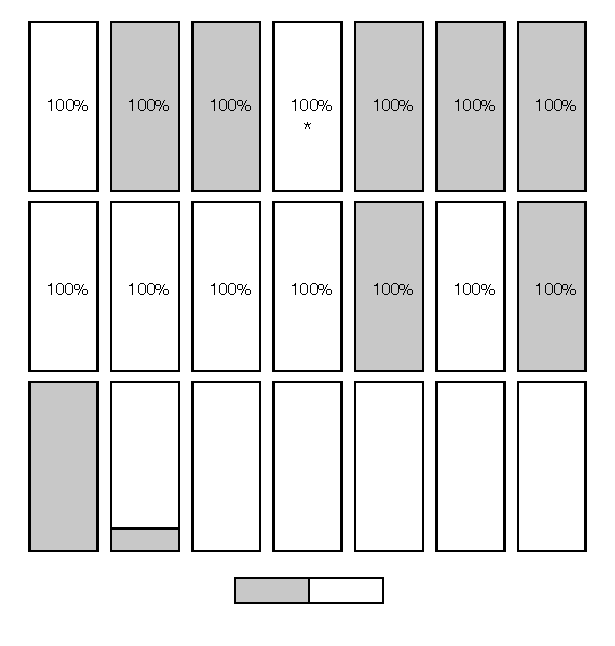
\includegraphics[width=4.5cm]{figs/Classific}
   \end{tabular}
 \end{tabular}
 \caption{\textrm{%
    Results for the 21 breast cancer data. A presents the five
    signatures obtained for the highest NMF model rank according to the
    BIC score presented in B. Signatures are labelled according to the
    order induced by the total signature exposure defined as $\hat e_n =
    \sum_{j} \hat e_{nj}$, with $S_1$ being the most exposed
    signature. \textcolor{red}{Mention the rescaling so that sum of bars
    equals 1?}  Bars are located at the MCMC sample median,
    i.e. $\widehat P$, while other horizontal level marks are located
    at the sample percentiles: *, *, *, and *.
    B: values for the BIC$(\theta^{(r)}_N)$, $1 \leq r \leq R$ obtained at
    various NMF ranks, $N$. C: Differential exposure scores - signatures
    showing median of log-p-values above thresholds were selected as
    differentially active among groups, and labels show group where they
    were most active.  Dashed horizontal lines are located at 
    the levels 0.05, 0.01 and 0.001. D: Classifications
    obtained for each breast cancer genome based on the remaining 20
    samples. The sample marked as `*' was the only
    misclassification found, `wt' stands for wild type BRCA1/BRCA2
    condition. Percentages show the correct classification proportion
    \textcolor{red}{RD: please confirm this last phrase}.
  }
 }\label{fig:bcancer} 
\end{figure*}
\subsection{The 21 breast cancer data}
The analysis of the 21 breast cancer data with opportunities revealed
5 distinct signatures (Figure~\ref{fig:bcancer}.A) that agree well
with existing knowledge as documented in Sanger's catalogue of
somatic cancer mutations (COSMIC, 
\url{http://cancer.sanger.ac.uk/cosmic/signatures}), and also in
\cite{HEN} and \cite{ANat}. The number of signatures necessary to
describe the data was obtained by considering the median BIC value out
of the set of values computed via MCMC samples. The BIC boxplots
obtained by varying $N$ from 1 to 12 are shown in
Figure~\ref{fig:bcancer}.B. Signatures $S_1$ and $S_5$ (respectively
signature 2 and 13 in COSMIC) are attributed to activity of the APOBEC
family of cytidine deaminases.  Signature $S_2$ (signature 1 in
COSMIC) is associated with a process initiated by the spontaneous
deamination of 5-methylcytosine and it correlates with patient age at
cancer diagnosis. Signature $S_3$ (signature 3 in COSMIC) is
associated with failure of DNA double-strand break-repair by
homologous recombination. Signature $S_4$ is of unknown aetiology. 


Results for the differential exposure score obtained while grouping
the data into two categories defined by samples with and without
germinative mutations in BRCA1 and BRCA2 genes are presented in
Figure~\ref{fig:bcancer}.C. The proteins encoded by the genes BRCA1
and BRCA2 play important roles in maintaining genomic stability and
are involved in a variety of cellular processes such as damage
signalling and DNA repair (\citealp{LY}). Disruption of such processes
often leads to a rapid and widespread accumulation of somatic
mutations in cancer cells (\citealp{Ash}). DES highlights three
mutational signatures (Figure~\ref{fig:bcancer}: $S_3$-$S_5$), two of
these are associated with inactivating mutations in BRCA1/BRCA2 genes
and implicated to activity of APOBEC genes (Figure~\ref{fig:bcancer}:
$S_1$ and $S_3$,\footnote{\textcolor{red}{IT: really? Shouldn't this
be $S_1$ and $S_5$; please see paragraph above!}} respectively). Taken
together, this findings are consistent with existing knowledge and
thereby may help explain the failure in the response to DNA damage by
homologous recombination in BRCA-defective breast cancer. We conclude
that the DES method is quite effective at revealing genotype-phenotype
relationships between groups of interest.\footnote{\textcolor{red}{IT,
    RD: $S_4$, not in COSMIC, is} VERY \textcolor{red}{differentially
    exposed. Which samples are these? Do we have anything to say?}} 

A leave-one-out cross-validation strategy was applied to test our
classification approach by examining the same sample categories used
in the DES analysis. This study is motivated by the fact that patients
with mutational profiles similar to those found in genomes with
mutated BRCA genes could respond to treatments targeting defective DNA
double-strand break repair mechanisms (\citealp{Ash}).  Each one of
the 21 genome samples had its label removed and was then subsequently
classified based on the remaining 20 samples.  Results are shown in
Figure~\ref{fig:bcancer}.D. Only one sample carrying a mutation at the
BRCA1 gene was misclassified, thus attesting the efficiency of our
classification approach.

\subsection{Simulation study}
Synthetic data sets mimicking real observations were assembled by
taking a group of four mutational signatures commonly found in breast
cancer genomes. These include the signatures 1, 2, 3 and 13 described
in Sanger's catalogue, also found by our analysis of the 21 breast
cancer data. Throughout, let $\widetilde P$ denote the resulting
signature matrix.  The exposures are generated by maximising the
likelihood $\mathcal L(\theta; m)$ for a given data sample $m$ with
respect to the exposure matrix $E$ by assuming the data as being
generated by $\widetilde P$. The maximisation of the likelihood in
($s_1$) with $P$ fixed at $\widetilde P$ is achieved by using the
\texttt{nlopt} package in R, but it may also be made by using
\cite{LS} multiplicative update algorithm to solve~(\ref{eqn:NMF}). A
matrix of simulated mutation counts $\widetilde m$ is finally
generated by sampling each entry $\widetilde m_{ij}$ from a Poisson
distribution with rate $(\widetilde P\widetilde E\circ W)_{ij}$.


A synthetic data set $\widetilde m$ generated by using the 21 breast
cancer data set was considered to compare the estimates for $\theta$
produced by our method and by those in \cite{A} and \cite{FICMV}. We
refer to these two alternative methods respectively as ANZ and EMu.
The same data set was analysed 100 times by each of the three
methods. All of the analyses made with \texttt{signeR} correctly
estimated four signatures. Only nine of the analyses performed by EMu
detected four signatures, the other 91 analyses estimated three.  The
accuracy of both methods was compared by the sum of squared errors
between $\widetilde P$ and the estimated signature matrix $\widehat
P$, defined as the squared Frobenius norm $\|\widetilde P - \widehat
P\|_F^2 = \sum_{in} |\widetilde P_{in} - \widehat
P_{in}|^2$\footnote{\textcolor{red}{RD: will $1 - \|\widetilde P -
\widehat P\|_F^2\, \big/\, \|\widehat P\|_F^2$ enhance the
coparizon?}}. Only those runs where EMu correctly estimated the
dimension of $P$ where included. These results are presented in
Figure~\ref{fig:synth_SSE}. Clearly, the estimates produced by
\texttt{signeR} are more ($p<*$) accurate than those obtained by EMu
or by ANZ ($p<*$). The median for the sum of squared errors obtained
with the analyses of \texttt{signeR} is *, while those for ANZ and
EMu's runs are respectively * and *.\footnote{\textcolor{red}{RD:
perhaps put the variances (or standard deviations)}}.

Further insights into the differences among the methods can be gained
by inspection of the likelihood at the estimates for $P$ and $E$,
despite of \texttt{signeR} being not just a likelihood maximisation
technique. The estimates obtained by EMu cluster about two different
likelihood values (see Figure~\ref{fig:synth_LLh}), the lower one is
identified with those runs where only three signatures are found and
the higher with those instances with four signatures. The estimates
obtained for \texttt{signeR} cluster at a single likelihood
value\footnote{\textcolor{red}{RD: Maybe we can mention that the value
is bellow one of EMu's because we have chosen to stay with the median
--not the mode (do you agree?)}}. These results reveal the stability
of \texttt{signeR} as opposed to EMu and AN-Z. It is well known that
the optimisation approach to NMF, as posed by~(\ref{eqn:NMF}), is
strongly sensitive to the initial condition because of high
dimensionality and because (\ref{eqn:NMF}) does not have a unique 
global minimum. Several initialisation strategies have been suggested
in the optimisation literature, see for instance \cite{LNACDarXiv,
BG, BBLPP}, but none of these where considered by \cite{FICMV} nor
\cite{A}.

\textcolor{red}{Further details about the repoducibility of the
  analyses in this section are presented as supplementary material (Figures~*, *).}

\begin{figure}  
 \centering
   \includegraphics[width=6cm]{figs/Simulation_signeR_vs_EMu_boxplot_SSE}
  \caption{\textrm{%
    Sum of squared errors for the estimated signature matrix obtained
    by \texttt{signeR}, AN-Z and EMu for a synthetic data set. 
   }
  }
  \label{fig:synth_SSE}
\end{figure}
\begin{figure}  
 \centering
  \includegraphics[width=6cm]{figs/Simulation_signeR_vs_EMu_histogram_LLh_same_axis}
  \caption{\textrm{%
   Histogram of Log likelihood values at the estimates for $P$ and $E$
   obtained by the analysis of a 4 signatures synthetic data set via
   \texttt{signeR} and EMu.
   }
  }
  \label{fig:synth_LLh}
\end{figure}

\section{Discussion}
The concept that many cancers acquire a mutator phenotype at different 
intensities is well accepted. Therefore, the ability to detect 
mutational signatures may provide insights about the development of
tumours. Here, we have outlined signeR, it employs a different and 
novel approach to deciphering mutational signatures, and featuring a
number of advantages when compared with others approaches. First, it
xxx $\ldots$ Second, xxx and Third $\ldots$ 


\texttt{signeR} is robust. It requires minimal intervention from part
of the user, but it also allows the incorporation of prior information
into the modelling. This justifies in part the empirical
approach. Mention that this reduces considerably the number of
parameters that have to be specified: from $2(KN+NG)=1170$ hyper
parameters down to 6.


\texttt{signeR} considers the model selection problem
robustly. Elaborate on the model selection problem to NMF --there is
space for improvement. Close.

\section*{Funding}
This work was partially supported by Funda\c{c}\~ao de Apoio a
Pesquisa do Estado de S\~ao Paulo (FAPESP), grant $\ldots$. 

%\vspace*{12pt}

%\bibliographystyle: natbib, achemnat, plainnat, abbrv, plain
\bibliographystyle{bioinformatics} 
\bibliography{bnmf}
\end{document}
%=-=-=-=-=-=-=-=-=-=-=-=-=-=-=-=-=-=-=-=-=-=-=-=-=-=-=-=-=-=-=-=-=-=
At hyperpriors section:

Maybe we have to justify why all this was made. The reason is to
reduce the dependency on a large number of free hyperparameters for
the model choice approach, i.e. the prior depends upon the
values of the hyperparameters if we don't integrate them out: for
$N=5$, $G=21$, $K=96$ we have $2(KN+NG)=1170$ (hyper)parameters to
set. With the hierarchical model, we are able to reduce the free
parameters down to 6.

\begin{enumerate}
\item[\textbf{1}.] Set $u = 0$ and initialise $\eta^{(0)}$ as
  $\eta^{(0)} = (1, \ldots, 1)$.
\item[\textbf{2}.] Initialise $Z^{(0)}$, $\theta^{(0)}$, $\psi^{(0)}$
  by sampling according to the hierarchical model, that is
  \begin{align*}
     &\psi^{(0)} \sim p(\psi | \eta^{(0)}) &\ 
        &\text{hyperprior}\\ 
     &\theta^{(0)} \sim p(\theta | \psi^{(0)}) &\ 
        &\text{prior}\\
     &Z^{(0)} \sim p(Z, M|\theta^{(0)}) &\ 
        &\text{complete data likelihood}
  \end{align*}
  Alternatively, the values for $\theta^{(0)}$ may be set by solving 
  (\ref{eqn:NMF}) via the NMF package from within R, see
  \citealp{GS}.
\item[\textbf{3}.] Iterate the Gibbs sampler to generate the sequence
 $\big(Z^{(r)}, \theta^{(r)}, \psi^{(r)}\big)$, $r = 1, \ldots, R$.
\item[\textbf{4}.] Update $\hat\eta^{(u)}$ according to the Monte
  Carlo EM formula (\ref{eqn:MCEM}) and set $u = u+1$. Return to step
\textbf{3} until $\big\|\hat\eta^{(u)} - \hat\eta^{(u-1)}\big\|_\infty  
\leq 0.05$ or $u > 100$. 
\item[\textbf{5}.] Set $\hat\eta = \hat\eta^{(u)}$ and then iterate
  the Gibbs sampler to obtain the final sequence of samples
  $\big(Z^{(r)}, \theta^{(r)}, \psi^{(r)}\big)$, $r=1, \ldots,
  R$. 
\end{enumerate}

Let $\delta = 2^d$ for $d \in \mathbb N$ such that $\frac{1}{8}T <
\delta \leq \frac{1}{4}T$ and then let $\mathcal T = \{1, \delta, 
2\delta, \ldots, T\}$.
\begin{enumerate}
\item Set $k^* = \big\{k \in \mathcal T: \overline{\text{BIC}}_k
  \geq \overline{\text{BIC}}_q, q \in \mathcal T\big\}$.
\item Set $\delta = 2^d/2$ and  then $\mathcal T = \{k^*-\delta, k^*, 
  k^*+\delta\}$.
\item Repeat steps {\bf 1}. and {\bf 2}. until $\delta=1$.
\item Set $N = k^*$.
\end{enumerate}

%\begin{enumerate}
%\item[\textbf{1}.] Limits for model rank are user-defined or set as 
%$1\leq rank \leq T$.
%\item[\textbf{2}.] Set \textit{range} = maximum\_rank - minimum\_rank
%  + 1.
%\item[\textbf{3}.] Set \textit{step} = $2^d$ for an integer \textit{d}
%  such that 
%$range/8 < step \leq range/4$.
%\item[\textbf{4}.] Evaluate rank = 1, 1 + \textit{step}, 1 +
%2*\textit{step}, ..., keeping the rank corresponding to the biggest
%median BIC found  (let us call it r\_optimum). The algorithm continues
%until it runs out of possibilities or evaluates two consecutive ranks
%for  which the median BICs are less then the biggest of those values 
%found so far.
%\item[\textbf{5}.] Update \textit{step} to half of its previous value.
%\item[\textbf{6}.] Evaluate rank = r\_optimum - \textit{step} and 
%rank = r\_optimum + \textit{step}, updating r\_optimum whenever needed.
%\item[\textbf{7}.] Return to 5 and iterates until \textit{step}=1.
%\item[\textbf{8}.] Select the final r\_optimum as the number of
%mutational signatures, $N$.
%\end{enumerate}

%%% Local Variables:
%%% mode: latex
%%% TeX-master: t
%%% End: